% IEEE Computer Society journal format for the TPDS manuscript.
% Based on the official IEEEtran bare_jrnl_compsoc.tex (V1.4b).
% Original ACM/APNet version is preserved in backups/acm-before-ieee/.
\documentclass[10pt,journal,compsoc]{IEEEtran}
\usepackage[T1]{fontenc}
\usepackage{graphicx}
\usepackage{amsmath,amssymb}
\usepackage[nocompress]{cite}
\usepackage[caption=false,font=footnotesize,labelfont=sf,textfont=sf]{subfig}
\usepackage[inline]{enumitem}
\usepackage{booktabs}
\usepackage{tabularx}
\usepackage{tikz}
\usetikzlibrary{arrows.meta,positioning}
\usepackage[hidelinks]{hyperref}

% Prefer one single-column top float; allow explicit top stacks where needed.
\setcounter{topnumber}{1}
\renewcommand{\topfraction}{0.85}

\begin{document}

\title{DuoGran: Dual-Granularity Load Balancing for RDMA Networks}

\author{Hong~Wang, Jinhao~Luo, Chang~Yu, Jingrong~Wang, and~Kaiyang~Liu%
\IEEEcompsocitemizethanks{%
\IEEEcompsocthanksitem Hong Wang, Jinhao Luo, Jingrong Wang, and Kaiyang Liu are with Memorial University of Newfoundland, St. John's, NL, Canada.\protect\\
E-mail: hongw@mun.ca; jinhaol@mun.ca; jingrongw@mun.ca; kaiyangl@mun.ca.
\IEEEcompsocthanksitem Chang Yu is with Nanjing University, Nanjing, China.\protect\\
E-mail: alicecyu@smail.nju.edu.cn.}}

\markboth{IEEE Transactions on Parallel and Distributed Systems}%
{Wang et al.: DuoGran: Dual-Granularity Load Balancing for RDMA Networks}

\IEEEtitleabstractindextext{%
\begin{abstract}
Load balancing in lossless remote direct memory access networks aims to optimize traffic distribution without incurring excessive packet reordering. We observe that priority-based flow control creates large gaps across pause boundaries. However, increasing path congestion can enlarge the delay difference between the current path and faster alternatives without producing a comparable increase in arrival gaps. Therefore, the order-preserving rerouting opportunities provided by natural gaps diminish as the current path congestion increases. To address these challenges, we propose DuoGran, a dual-granularity load-balancing scheme that combines flowlet-based and protected subflow-based rerouting. DuoGran dynamically adjusts the per-connection flowlet timeout to exploit natural inter-packet gaps for rerouting without waiting for congestion on the current path. When the current path becomes congested, it selectively enables protected subflow rerouting, using buffering at the destination top-of-rack (ToR) switch to preserve in-order delivery. Large-scale simulations and hardware testbed experiments show that DuoGran reduces average and P99 flow completion times by up to [XX\%] and [YY\%], respectively, and lowers the P99 destination-ToR reordering-buffer occupancy by approximately 60.1\% compared with state-of-the-art schemes.
\end{abstract}

% Preserve the original ACM subject classification as an IEEE index term.
\begin{IEEEkeywords}
RDMA, Load Balancing, Flowlet, Subflow, Data Center Networks
\end{IEEEkeywords}}

\maketitle
\IEEEdisplaynontitleabstractindextext

\section{Introduction}
Efficient load balancing is essential to realizing the performance benefits of remote direct memory access (RDMA) in data centers. Equal-Cost Multi-Path (ECMP)~\cite{ECMP} distributes flows across available paths using congestion-oblivious hashing, which may place multiple elephant flows on the same path. Such hash collisions can increase queueing delay while leaving other paths underutilized~\cite{HPCC, Meta}. Balancing traffic across available paths is therefore important for sustaining RDMA performance.

However, distributing packets of a connection across multiple paths can incur packet-reordering penalties. Packet-spraying schemes~\cite{MPRDMA, Eunomia, PLB, Proteus} evenly spread packets across available paths, but differences in path delay can cause out-of-order arrivals. For RDMA transports using Go-Back-N (GBN) recovery, such arrivals can trigger retransmissions and increase flow completion time (FCT)~\cite{Conweave, Seqbalance}. Selective Repeat can accommodate out-of-order delivery, but requires RDMA network interface cards (RNICs) to maintain additional state to track received packets and buffer packets to restore their order~\cite{IRN, SRNIC}. Load balancing must therefore determine both when to change paths and how to preserve packet order or accommodate reordering.

Congestion-triggered subflow schemes~\cite{Conweave, Hopper, RoCELet} reroute traffic after detecting congestion on the current path. However, such reactive rerouting may not exploit spare capacity on alternative paths in time. Traffic can remain concentrated on a heavily loaded path before rerouting is triggered or takes effect, allowing load imbalance to persist.



These limitations motivate exploiting rerouting opportunities beyond congestion-triggered path changes. Our observations show that priority-based flow control (PFC) pauses can create large inter-packet gaps in otherwise continuous RDMA streams, providing opportunities to redistribute traffic across paths. However, traditional flowlet-based schemes such as CONGA and LetFlow~\cite{Conga, Letflow} use a static timeout, making it difficult to exploit these gaps effectively. A timeout that is too small risks packet reordering, whereas one that is too large misses otherwise usable rerouting gaps. To address this tuning challenge, we dynamically adjust the per-connection flowlet timeout based on the delays of the current and candidate paths.

However, relying solely on PFC-induced inter-packet gaps may not provide sufficient opportunities to reroute traffic away from congested paths in a timely manner. As congestion increases the delay difference between the current path and a faster alternative, arrival gaps do not necessarily grow accordingly. Consequently, natural opportunities for order-preserving rerouting diminish as congestion on the current path increases.

These observations motivate DuoGran, a dual-granularity load-balancing scheme that combines flowlet-based and protected subflow-based rerouting. Dynamic per-connection timeouts enable flowlet rerouting by exploiting PFC-induced inter-packet arrival gaps as natural switching boundaries, without waiting for congestion on the current path. When the current path becomes congested, natural gaps may no longer provide sufficient opportunities for order-preserving switching because of the larger delay difference between the current and candidate paths. DuoGran then selectively enables protected subflow rerouting, using buffering at the destination top-of-rack (ToR) switch to preserve in-order delivery.



\begin{table}[t]
    \centering
    \caption{Rerouting granularity, flowlet timeout, and reordering support of representative schemes.}
    \label{tab:lb_comparison}
    \footnotesize
    \setlength{\tabcolsep}{3pt}
    \renewcommand{\arraystretch}{1.15}
    \begin{tabularx}{\columnwidth}{@{}l>{\raggedright\arraybackslash}p{0.18\columnwidth}>{\raggedright\arraybackslash}p{0.22\columnwidth}>{\raggedright\arraybackslash}X@{}}
        \toprule
        \textbf{Scheme} & \textbf{Granularity} & \textbf{Flowlet timeout} & \textbf{Reordering support} \\
        \midrule
        ECMP~\cite{ECMP} & Flow & --- & None \\
        CONGA~\cite{Conga} & Flowlet & Static & None \\
        LetFlow~\cite{Letflow} & Flowlet & Static & None \\
        ConWeave~\cite{Conweave} & Subflow & --- & Destination ToR \\
        MP-RDMA~\cite{MPRDMA} & Packet & --- & RNICs \\
        DuoGran & Flowlet + subflow & Dynamic per connection & Destination ToR (selective) \\
        \bottomrule
    \end{tabularx}
\end{table}

The contributions of DuoGran include the following:
\begin{itemize}
    \item We identify PFC-induced inter-packet gaps as natural rerouting opportunities and show how increasing path-delay differences under congestion limit their use for order-preserving switching.
    \item We propose DuoGran, a dual-granularity load-balancing scheme that combines flowlet rerouting with dynamic per-connection timeouts and selective protected subflow rerouting, using destination-ToR buffering to preserve in-order delivery.
    \item Through large-scale simulations and hardware testbed experiments, we demonstrate reductions of up to [XX\%] and [YY\%] in average and P99 FCT, respectively, and approximately 60.1\% in P99 reordering-buffer occupancy compared with state-of-the-art schemes.
\end{itemize}

\section{Related Work}
\subsection{Load Balancing in Lossless RDMA}



\noindent
Beyond flow-based ECMP, existing load-balancing schemes for lossless RDMA can be broadly categorized as packet-spraying, flowlet-based, or subflow-based schemes. Table~\ref{tab:lb_comparison} summarizes representative schemes, their rerouting granularities, flowlet timeout policies, and reordering support.

\noindent
\textbf{Packet-spraying schemes} distribute traffic at packet granularity to exploit multiple paths. However, due to varying levels of congestion across paths, packets can arrive at the destination RNIC out of order. For RNICs using GBN recovery, out-of-order arrivals can trigger retransmissions and cause subsequent packets to be discarded until the missing packet is received \cite{Conweave}. 

Fine-grained multipath forwarding therefore requires either mechanisms that prevent reordering or support that accommodates out-of-order arrivals, as discussed in Sec.~\ref{sec:related_reordering}.

\noindent
\textbf{Subflow-based schemes \cite{Hopper, RoCELet, Reunion}} trigger path changes in response to congestion and use additional mechanisms to preserve packet order. However, by the time congestion signals reach the source, queues have already built up, triggering PFC pause frames that can lead to head-of-line blocking or deadlocks \cite{PFC_bad}. Some schemes also introduce waiting periods to preserve packet order during path changes. Hopper~\cite{Hopper} delays path switching, whereas RoCELet~\cite{RoCELet} temporarily suspends transmission, potentially increasing FCT.

\noindent
\textbf{Flowlet-based schemes} such as CONGA and LetFlow~\cite{Conga, Letflow} exploit natural inter-packet gaps to switch paths. However, selecting an appropriate static timeout is challenging in continuous RDMA streams. A small timeout risks packet reordering, whereas a large one misses usable rerouting gaps. HF$^2$T~\cite{HF2T} addresses the scarcity of sufficiently large gaps by inserting idle intervals at the hosts, but the added waiting can increase FCT. DuoGran instead exploits existing arrival gaps through dynamic per-connection timeout tuning.

\subsection{Reordering Support for Multipath RDMA}
\label{sec:related_reordering}

Rerouting before a sufficiently large inter-packet gap becomes available requires mechanisms to accommodate out-of-order arrivals. Such support can be implemented in RNICs or within the network.

\noindent
RNIC-based reordering support must balance tracking capacity, memory consumption, and processing latency. MELO~\cite{MELO} separates packet-data storage from reception metadata and dynamically allocates bitmap blocks from a shared pool. LEFT~\cite{LEFT} addresses the access latency of shared bitmap structures through bitmap caching and packet gathering. Eunomia~\cite{Eunomia} further explores on-demand allocation and a hybrid circular--linear bitmap, enabling dynamic expansion without remapping existing entries and indexed access without linked-list traversal.

MP-RDMA~\cite{MPRDMA} takes a complementary approach by controlling the degree of reordering at the sender. It suppresses traffic on lagging paths when acknowledgment feedback indicates excessive reordering, thereby limiting the bitmap size needed to track out-of-order packets. Deploying these mechanisms requires programmable RNICs to support custom packet processing and state management, limiting their applicability to fixed-function commercial RNICs.

ConWeave~\cite{Conweave} provides in-network reordering support using programmable switches, buffering new-path packets at the destination ToR while waiting for old-path traffic. Its congestion-triggered rerouting does not require a natural inter-packet arrival gap. When switching from a slower path to a faster one, a larger delay difference can increase destination buffering demand under otherwise comparable traffic conditions. DuoGran builds on in-network reordering but focuses on when to invoke it. It exploits natural arrival gaps through delay-aware flowlet switching and selectively uses destination-ToR buffering for protected subflow rerouting on congested paths, aiming to limit the traffic that requires reordering support.

\subsection{Summary}
\noindent
Existing approaches in lossless RDMA face a tradeoff between improving path utilization and limiting packet-reordering penalties. DuoGran dynamically adjusts the per-connection flowlet timeout according to changing path conditions, exploiting natural inter-packet gaps to redistribute traffic and alleviate load imbalance. To address the diminishing opportunities for order-preserving rerouting as path congestion increases, DuoGran selectively enables protected subflow rerouting when the current path is congested, using destination-ToR buffering to preserve in-order delivery.



\section{Background and Motivation}
\label{sec:background}

\subsection{Limitations of Congestion-Triggered Rerouting}
\label{sec:conweave_motivation}
Congestion-triggered rerouting responds to congestion on the current path, but does not necessarily redistribute traffic whenever another path offers spare capacity. Load imbalance may therefore persist before rerouting is triggered or takes effect. We examine this limitation through local uplink measurements under ConWeave.

\begin{figure}[!t]
    \centering
    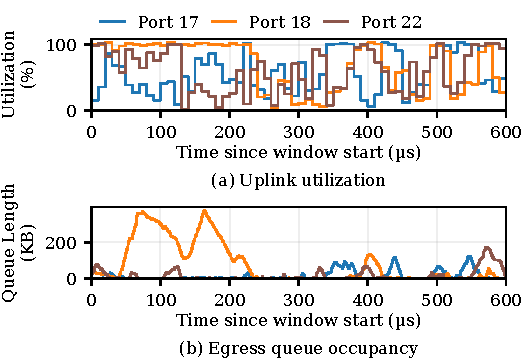
\includegraphics[width=\columnwidth]{figures/conweave_uplink_queues.pdf}
    \caption{The plots show the utilization and egress queue occupancy of selected uplinks at a source ToR under ConWeave. Link utilization is measured over 10-$\mu$s windows, and queue occupancy is sampled every 1~$\mu$s.}
    \label{fig:conweave_uplink_queues}
\end{figure}

Figure~\ref{fig:conweave_uplink_queues} shows utilization and egress queue occupancy on selected source-ToR uplinks under ConWeave with the AliStorage workload over a 600-$\mu$s interval. Under congestion-triggered rerouting, traffic can remain concentrated on a heavily queued uplink while another uplink is underutilized. For example, at 80~$\mu$s into the displayed interval, port 18 holds approximately 344~KB of queued data and reaches 99.7\% utilization in the following 10-$\mu$s window. In contrast, port 17 has an empty queue and only 22.5\% utilization over the same window, leaving substantial transmission capacity unused. This local imbalance illustrates that congestion-triggered subflow rerouting may leave available uplink capacity underutilized.

This observation motivates exploiting opportunities to redistribute traffic beyond congestion-triggered rerouting. The following subsections examine natural inter-packet gaps as one source of such opportunities, and why these gaps become less useful as path latency differences grow.

\subsection{Natural Rerouting Opportunities in Lossless RDMA}
\label{sec:pfc_gaps}
\setcounter{dbltopnumber}{2}
Hardware-paced RDMA streams typically have short inter-packet arrival gaps, making natural flowlet opportunities difficult to find~\cite{HF2T, Conweave}. Nevertheless, PFC pauses can introduce large gaps into otherwise continuous streams. These gaps provide opportunities to switch to a faster path while preserving packet order.

\setcounter{dbltopnumber}{2}




\begin{figure}[!t]
    \centering
    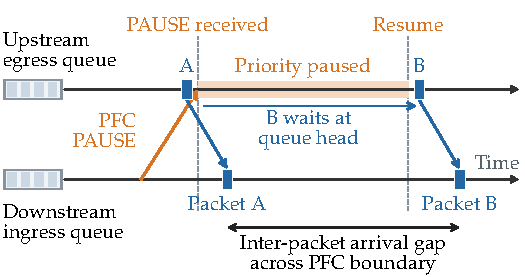
\includegraphics[width=\columnwidth]{figures/pfc_boundary_explained.pdf}
    \caption{Consecutive same-flow packets A and B are transmitted before the pause and after resumption, respectively. The PFC pause creates an inter-packet arrival gap at the downstream switch.}
    \label{fig:pfc_boundary_explained}
\end{figure}

\begin{figure}[!t]
    \centering
    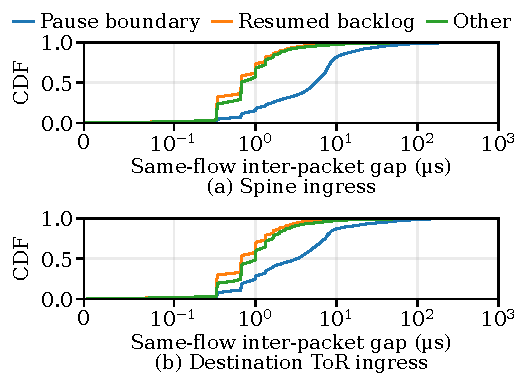
\includegraphics[width=\columnwidth]{figures/conga_pfc_boundary_gaps.pdf}
    \caption{Same-flow inter-packet arrival-gap CDFs under CONGA on a 128-host leaf--spine topology with the all-to-all AliStorage workload, measured at (a) spine ingress and (b) destination-ToR ingress.}
    \label{fig:conga_pfc_boundary_gaps}
\end{figure}

\begin{figure*}[!t]
    \centering
    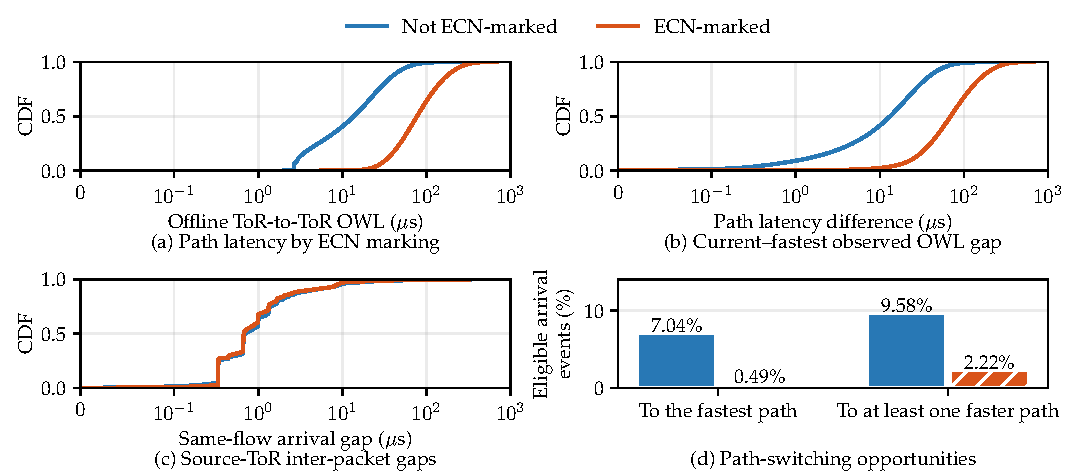
\includegraphics[width=\textwidth]{figures/conga_four_panels.pdf}
    \setlength{\abovecaptionskip}{0pt}
    \caption{Path latency and potential rerouting opportunities under CONGA, grouped offline by destination-ToR ECN marking. (a) Offline path one-way latency (OWL). (b) Current-path latency minus the fastest observed candidate's estimated latency. (c) Source-ToR arrival gaps. (d) Observed events satisfying $g>\Delta L$.}
    \label{fig:conga_offline_opportunities}
\end{figure*}

\noindent
\textbf{Rerouting opportunities across PFC pause boundaries.}
When ingress queue occupancy exceeds a configured threshold, the downstream switch sends PFC pause frames to suspend the corresponding priority queue at the upstream switch, causing packets to accumulate~\cite{DCQCN}. Transmission resumes when a resume frame arrives or the pause timer expires. This interruption can create large inter-packet arrival gaps at the downstream switch.

Figure~\ref{fig:pfc_boundary_explained} illustrates a PFC-induced inter-packet arrival gap. Packets A and B are consecutive packets of the same flow spanning a pause boundary. A is the last packet of that flow transmitted before the upstream egress queue pauses, and B is the first transmitted after it resumes. B is already queued at the upstream switch when transmission resumes. The pause separates their transmissions, creating a gap between their arrival times at the downstream switch.



Figure~\ref{fig:conga_pfc_boundary_gaps} demonstrates this effect in the CONGA experiment. At spine ingress, pause-boundary gaps have a median of 5.538~$\mu$s and a P99 of 98.911~$\mu$s. Destination-ToR ingress shows the same pattern. PFC pause boundaries provide substantially larger arrival gaps, whereas packets accumulated during the pause arrive in closely spaced bursts after resumption. These resumed-backlog packets are already queued when transmission resumes. Their arrival gaps at spine ingress have a median of only 0.670~$\mu$s and a P99 of 9.442~$\mu$s. Thus, the large gap across a pause boundary is followed by much shorter gaps within the released backlog.

These gaps provide potential rerouting opportunities. However, traditional flowlet-based schemes such as CONGA~\cite{Conga} and LetFlow~\cite{Letflow} use a static timeout, whose tuning is challenging in continuous RDMA streams. A timeout that is too small risks packet reordering, whereas one that is too large misses otherwise usable rerouting gaps. A fixed timeout cannot accommodate the different and time-varying delay differences between current and candidate paths. This motivates adjusting each connection's timeout according to the measured path delays.



\subsection{Diminishing Rerouting Opportunities}
\label{sec:conga_offline_gaps}

Dynamic timeout tuning can exploit inter-packet arrival gaps to enable path changes that a conservative static timeout would miss. However, even with a timeout adapted to the current and candidate paths, order-preserving switching remains constrained by their delay difference. Switching to a substantially faster path offers a larger potential latency reduction but requires a larger arrival gap to prevent packet reordering. As congestion increases this delay difference without a comparable increase in arrival gaps, natural-gap-based rerouting may not move traffic away from congested paths in time.

Figure~\ref{fig:conga_offline_opportunities} examines CONGA on a 128-host leaf--spine topology with the AliStorage workload at 80\% load. We group samples offline by the Congestion Experienced (CE) marking in the Internet Protocol header at destination-ToR ingress and compare path delays with same-flow arrival gaps at the source ToR.\footnote{Path OWL is measured from source-ToR arrival to destination-ToR arrival. Candidate latency is estimated from a reference packet's transit time on that path within $\pm5~\mu$s of the current source arrival. No sampled packet carries CE at source-ToR ingress.}

\noindent
\textbf{Larger path-delay differences without larger arrival gaps.}
Figure~\ref{fig:conga_offline_opportunities}(a) shows that CE-marked samples tend to have higher path OWL. Figure~\ref{fig:conga_offline_opportunities}(b) compares the current path with the fastest observed alternative, using $\Delta L=L_{\mathrm{current}}-\widehat{L}_{\mathrm{fastest}}$. Among events with an observed faster alternative, the median difference is 62.080~$\mu$s for CE-marked samples, versus 12.393~$\mu$s for samples not marked CE. In contrast, Figure~\ref{fig:conga_offline_opportunities}(c) shows a median arrival gap of 0.666~$\mu$s in both groups, with both distributions concentrated at short gaps. Thus, the larger delay differences between high-latency paths and faster alternatives offer greater potential latency reductions, but are not accompanied by correspondingly larger source-ToR inter-packet arrival gaps.

\noindent
\textbf{Fewer observed opportunities for order-preserving switching.}
Under an idealized delay comparison, order-preserving switching to a faster path requires the source-ToR inter-packet arrival gap $g$ to exceed the path-delay difference $\Delta L$. Larger delay differences without correspondingly larger arrival gaps therefore leave fewer opportunities for such switching. Figure~\ref{fig:conga_offline_opportunities}(d) reports the fraction of arrival events whose gaps exceed the delay difference between the current path and a faster alternative. When targeting the fastest observed path, this fraction decreases from 6.10\% for samples not marked CE to 0.41\% for CE-marked samples. Allowing any observed faster path gives 7.90\% and 1.72\%, respectively. These results indicate that natural gaps offer fewer observed opportunities to switch away from congested paths while preserving packet order. This limitation motivates protected subflow rerouting, which uses destination-ToR buffering to preserve in-order delivery when the available gaps are insufficient for flowlet switching.

\subsection{Summary}
PFC-induced inter-packet arrival gaps provide rerouting opportunities, and dynamic per-connection timeouts account for changing path-delay differences to exploit gaps that a conservative static timeout would miss. However, when congestion increases path-delay differences without a comparable increase in arrival gaps, opportunities for order-preserving flowlet switching become more restrictive. This motivates combining dynamic flowlet switching with protected subflow rerouting: on congested paths, existing gaps can enable an earlier switch, with destination-ToR buffering preserving packet order during the handoff.

\section{Design}
Building on these observations, DuoGran combines delay-aware flowlet switching with selective, gap-qualified early rerouting. Path selection and measurement reside at the ToRs. The exploration-first policy applies when a packet creates a new flow-table entry, including after the original entry has aged out. For an existing entry, the source first evaluates the ordinary improvement and path-pair timeout conditions. If these do not admit a change, an invalid current path may qualify for a protected early switch under the conditions in Sec.~\ref{sec:selective_handoff}. Otherwise, the current path is retained.

\subsection{Path Monitoring and Exploration-first Selection}
\label{sec:OWL_monitoring}
\label{sec:exploration}
DuoGran maintains path measurements and availability states at the source ToR to support initial path assignment and subsequent rerouting. It combines latency measurements with congestion feedback and prioritizes paths requiring reassessment when assigning new connections.

\noindent
\textbf{Path-delay measurement.} Each path $i$ maintains an \texttt{iswaiting} flag, initially set to 0. The source ToR initiates a measurement only when this flag is 0. It sets a measurement bit in a data packet, records its transmission timestamp $d_i^{\mathrm{trans}}$, sets \texttt{iswaiting} to 1, and establishes a reply deadline
\begin{equation}
    d_i^{\mathrm{exp}} = d_i^{\mathrm{trans}} + RTT_i^{\mathrm{base}} + \delta,
    \label{eq:measurement_deadline}
\end{equation}
where $RTT_i^{\mathrm{base}}$ is the base RTT measured under contention-free conditions and $\delta$ accommodates processing jitter. Paths with the same hop count and link characteristics share the same base RTT estimate.

Upon receiving the flagged packet, the destination ToR records its arrival timestamp $d_i^{\mathrm{rec}}$ and copies the forward-path identifier from the packet header. It returns both fields to the source ToR in an \texttt{OWL\_REPLY} control packet via ECMP. The source ToR computes the path OWL as
\begin{equation}
    L_i = d_i^{\mathrm{rec}} - d_i^{\mathrm{trans}},
    \label{eq:owl_measurement}
\end{equation}
and updates the latency change rate using consecutive measurements. With each sample time $t_i$ set to its transmission timestamp $d_i^{\mathrm{trans}}$, the change rate is
\begin{equation}
    r_i = \frac{L_i^{\mathrm{new}}-L_i^{\mathrm{old}}}
                   {t_i^{\mathrm{new}}-t_i^{\mathrm{old}}}.
    \label{eq:owl_rate}
\end{equation}
The first measurement uses zero rate; an equal-time sample retains the previous rate. The \texttt{iswaiting} flag is cleared only upon receiving the corresponding \texttt{OWL\_REPLY}, even if the reply deadline has expired. This ensures that each path has at most one outstanding measurement, limiting control-packet overhead and preventing overlapping requests from overwriting the recorded transmission timestamp. Active paths can be measured again once their replies arrive. In lossless RDMA, PFC prevents congestion-induced buffer overflow, protecting flagged packets and their replies from congestion-related drops.

\noindent
\textbf{Congestion feedback and timeout handling.} \texttt{ECN\_REPLY} explicitly reports congestion, whereas an \texttt{OWL\_REPLY} timeout can indicate potential congestion even before explicit congestion feedback arrives. When an arriving data packet carries a CE mark, the destination ToR generates a separate \texttt{ECN\_REPLY} control packet, copies the forward-path identifier from the data packet, and sends the reply back to the original source ToR. The source ToR uses this identifier to mark the affected path Invalid. If \texttt{OWL\_REPLY} does not arrive before $d_i^{\mathrm{exp}}$, the source ToR also marks the path Invalid.

\noindent
\textbf{Path-state management.} Each path is classified as Available, Invalid, or Unknown. All paths are initially Available, allowing transmission before measurements have been collected. Available denotes eligibility for selection rather than guaranteed congestion-free forwarding. Congestion feedback or a reply timeout makes the path Invalid for an interval $d_i^{\mathrm{unav}}$. When this interval expires, the path transitions to Unknown because elapsed time alone does not establish that congestion has subsided. A timely, non-congested measurement initiated after the invalid interval restores the path to Available; congestion feedback or another reply timeout returns it to Invalid.

\noindent
\textbf{Exploration-first selection.} For a new connection, DuoGran prioritizes Unknown paths eligible for probing, selecting among them in round-robin order. The connection's first packet serves as the flagged probe, allowing transmission to begin while reassessing the selected path. If no Unknown path is eligible, DuoGran selects an Available path, preferring the lowest measured OWL when measurements are available. Initially unmeasured Available paths remain eligible for assignment and are measured when selected. If neither choice provides a candidate, DuoGran uses a fallback path without changing its state. Exploration-first selection applies only to initial path assignment; subsequent path changes follow the dynamic flowlet and protected subflow rerouting policies described below. For these subsequent decisions, $A_{s,d}$ denotes the set of Available paths with OWL measurements between source ToR $s$ and destination ToR $d$.

\noindent
\textbf{Clock offsets.} DuoGran compares paths between the same source--destination ToR pair. A constant clock offset adds the same bias to their OWL measurements, preserving path ranking and cancelling in the delay difference between the current and candidate paths. It also cancels between consecutive measurements when computing latency changes. These calculations therefore tolerate a fixed clock offset, provided that it remains stable over the relevant measurement interval. Time-varying offsets can affect the estimates.

\subsection{Dynamic Per-connection Timeout Tuning}
\label{sec:dynamic_timeout}
As discussed in Sec.~\ref{sec:pfc_gaps}, PFC can create inter-packet arrival gaps across pause boundaries. DuoGran exploits these existing gaps by adapting the flowlet timeout to the current and candidate paths. The timeout combines their measured delay difference, a directional EWMA protection term, and a bounded local-queue correction to limit packet-reordering risk.

For an existing flow entry, let $c$ denote its current path and $g$ the interval since its previous packet arrived at the source ToR. If rerouting is disabled, the flow keeps $c$. Otherwise, the only candidate is
\begin{equation}
    b = \arg\min_{i\in A_{s,d}} L_i.
    \label{eq:best_path}
\end{equation}
Equal-OWL ties use the path identifier in the current implementation. If there is no available candidate, $b=c$, or the current path has no OWL measurement, the packet stays on $c$. Candidate ranking uses the latest OWL, not a predicted OWL. The policy does not scan other available paths if $b$ fails a rerouting check.

\noindent
\textbf{Predicted improvement:} Let $H_{s,d}$ be a configured prediction horizon, defaulting to the destination's base RTT. The estimated improvement from switching is
\begin{equation}
    I_{c,b} = L_c-L_b+H_{s,d}(r_c-r_b).
    \label{eq:improvement}
\end{equation}
The change is considered only when $I_{c,b}>I_{\min}$, where $I_{\min}=1~\mu\mathrm{s}$ is the minimum required latency improvement. The rates in this check assess the expected benefit, while the timeout below uses smoothed directional changes to account for reordering risk.

\noindent
\textbf{Directional EWMA protection:} An increasing delay on the current path can hold back earlier packets; a decreasing delay on the candidate can bring subsequent packets forward. Let $[x]^+=\max(0,x)$ and $\Delta L_{i,k}=L_{i,k}-L_{i,k-1}$ be the change between successive valid OWL samples on path $i$. We maintain separate exponentially weighted moving averages (EWMAs) for its upward and downward changes:
\begin{equation}
    \begin{aligned}
        U_{i,k} &= (1-\beta)U_{i,k-1}+\beta[\Delta L_{i,k}]^+, \\
        D_{i,k} &= (1-\beta)D_{i,k-1}+\beta[-\Delta L_{i,k}]^+,
    \end{aligned}
    \label{eq:directional_ewma}
\end{equation}
where $\beta=1/8$. The first sample initializes the reference OWL with $U_i=D_i=0$. Only samples with increasing transmission timestamps update these estimates; duplicate or older samples neither change the reference nor decay the estimates. The protection term is $G_{c,b}=2(U_c+D_b)$, combining the two directions that can reduce the separation between old-path and new-path packets. Both estimates have units of time, and candidate ranking continues to use the latest OWL.

\noindent
\textbf{Local-queue correction:} The source ToR also observes the current backlog at the egress port associated with each path. Let $q_i$ be the queued bytes for the arriving packet's priority multiplied by eight and divided by the port's line rate, rounded upward to whole nanoseconds. This snapshot is taken before the packet is enqueued. We use the bounded correction
\begin{equation}
    Q_{c,b}=\min\!\left(2~\mu\mathrm{s},\;\tfrac{1}{2}[q_c-q_b]^+\right).
    \label{eq:queue_correction}
\end{equation}
The weight and cap limit the added margin because the OWL sample may already reflect local queueing. The nonnegative correction cannot lower the timeout below its value without this term. This estimate covers the observed local backlog; it excludes PFC waiting time and downstream queues.

\noindent
\textbf{Timeout and switching decision:} The resulting timeout is
\begin{equation}
    \begin{aligned}
        T_{c,b}=\Bigl\lceil
        &\max\!\left(T_{\mathrm{floor}},[L_c-L_b+G_{c,b}]^++M\right) \\
        &{}+Q_{c,b}\Bigr\rceil_{\mathrm{ns}},
    \end{aligned}
    \label{eq:pair_timeout}
\end{equation}
where $T_{\mathrm{floor}}=M=1~\mu\mathrm{s}$, and $\lceil\cdot\rceil_{\mathrm{ns}}$ rounds upward to whole nanoseconds. The queue correction is added after applying the minimum gap. Ordinary flowlet rerouting requires both $I_{c,b}>I_{\min}$ and $g>T_{c,b}$. It is also blocked while the current local egress queue is PFC-paused. If the ordinary branch rejects a change, the source may still evaluate the protected early-rerouting conditions in Sec.~\ref{sec:selective_handoff}. The flow retains $c$ when neither branch admits a change.

The ordinary conditions apply whether $c$ is Available or Invalid; path invalidity and a local PFC pause are distinct states. An invalid current path is excluded from candidate selection, but its retained measurements still describe the path used by earlier packets. After every packet, the flow's last-arrival time is updated. A successful ordinary path change begins the next flowlet.

The timeout is calculated on demand from shared path state. OWL measurements, rates, and directional EWMAs are maintained per path rather than duplicated per connection; the local-queue term is read at the decision point. DuoGran stores neither a live timeout per flow nor a maximum-minus-minimum OWL gap across all ECMP paths. These estimates aim to reduce reordering risk but do not provide deterministic delay bounds: delayed feedback, future queue changes, and downstream pauses can still cause the actual packet delays to differ from the estimates.

\subsection{Selective Early Rerouting and Destination Buffering}
\label{sec:selective_handoff}

Holding packets that arrive ahead of earlier traffic requires buffer space and can introduce additional waiting at the destination ToR. This tradeoff motivates combining natural-gap-based switching with selective reordering support. Our use of destination-ToR reordering builds on the approach established by ConWeave~\cite{Conweave}. We adopt the principle of holding new-path packets until an old-path boundary permits their release; we do not claim destination buffering itself as a new contribution. The distinction pursued here is the policy for invoking this support: natural gaps and path-pair delay estimates govern ordinary switching, while explicit protection is reserved for selected early reroutes that cannot pass the ordinary timeout check.

In the current DuoGran implementation, this early branch requires an invalid current path, a same-flow arrival gap strictly greater than $2~\mu\mathrm{s}$, and a faster available candidate that passes the predicted-improvement check. It does not require the gap to exceed the full path-pair timeout. The source sends an END control packet along the old path and tags subsequent new-path data with a handoff identifier. The destination creates temporary state and holds new-path packets until the corresponding END and any preceding handoff boundaries have completed. The current implementation uses CLEAR and CLOSE control messages to retire the temporary state. Ordinary timeout switches outside an active handoff do not start this protection; switches within an active handoff remain covered by its boundary tracking.

The existing arrival gap gives old data a head start, but END is sent when the switch is selected and still traverses the old path. Therefore, gap-qualified early rerouting aims to limit buffering demand without assuming that every larger gap reduces the wait for END. Its protection also does not retroactively cover packets on historical paths preceding the handoff. Section~\ref{sec:dst_buffer_occupancy} reports the preliminary buffering comparison and its limitations.

\subsection{Implementation and Overhead Analysis}
\label{sec:implementation}
\noindent
\textbf{Forwarding and metadata:} The NS-3 implementation encodes the selected source route in a path identifier, tracks the hop index, and flags selected data packets for measurement using packet tags. Intermediate switches use the encoded route. Feedback carries path and timing information. Simulator tags do not establish a deployable wire format, so header placement and serialization overhead require a separate hardware design.

\noindent
\textbf{Shared state:} Each source ToR stores one path table per destination ToR. A dense array holds each path's measurement and control state once. Internal nodes of an implicit binary tree summarize the lowest available OWL and its path, available-path count, and earliest probe-eligible time. Only Unknown paths with no pending measurement are eligible for exploration. Expiration of an invalid interval makes a path Unknown but does not automatically restore its availability.

The per-flow table records the selected path and last packet-arrival time, with additional counters for simulator logging. It retains the existing inactivity-aging policy. OWL values and rates are shared by all flows using the same ToR-pair path; they are not duplicated per flow.

\noindent
\textbf{Algorithm complexity:} For $P$ paths to one destination, reading the best available path and available count from the root costs $\mathrm{O}(1)$. Cursor-based exploration and a path-state update cost $\mathrm{O}(\log P)$. The current path-identifier lookup also uses binary search, so a complete rerouting decision is not solely an $\mathrm{O}(1)$ root read. With $D$ destinations, up to $P$ paths per destination, and $F$ active flow entries, total state is $\mathrm{O}(DP+F)$. No separate sorted measurement set or global OWL extrema are needed.

\noindent
\textbf{Measurement overhead:} Probes reuse data packets, and each flagged packet requests a reply. Limiting each path to one pending reply bounds concurrent requests but does not establish negligible aggregate overhead; reply traffic grows with the number of actively monitored paths and their refresh frequency. When new-flow arrivals are sparse, unused paths may receive no new probes, although active paths continue to be measured. The current design does not add an autonomous packet generator or a new probe-retry timer.

\noindent
\textbf{Hardware scope:} The tree describes the C++ simulator implementation. A P4 realization would need fixed-size state, bounded pipeline operations, and a representation of the rate calculations suitable for the target. We do not infer line-rate operation or a concrete static random-access memory budget from the C++ data structure; these require target-specific implementation and validation.



\section{Performance Evaluation}
\noindent
\textbf{Draft evaluation status:} The FCT and PFC results in Sec.~\ref{sec:result} are retained from the earlier prototype, which used flow-size classification and a different timeout mechanism. They are historical reference results, not measurements of the revised exploration-first design in Sec.~\ref{sec:exploration}. Sections~\ref{sec:subflow_fct_ablation} and~\ref{sec:dst_buffer_occupancy} separately report a preliminary FCT ablation and a buffering experiment with the current DuoGran extension. A full evaluation of the revised design remains necessary before general performance gains can be claimed.


\subsection{Simulation Setup} 
The evaluation framework uses NS-3~\cite{ns3} and builds upon the open-source ConWeave simulator~\cite{Conweave}, which models a lossless RDMA stack. The offset maximum transmission unit is revised to 4096 bytes to accommodate the real-world 

\noindent
\textbf{Congestion control:} We employ DCQCN as the default congestion control algorithm since the commercial RNIC for lossless by default support it. All the parameters align with the open-sourced implementation in ConWeave.

\noindent
\textbf{Baselines and parameter tuning:} To evaluate DuoGran, we compare it against flow-based ECMP, flowlet-based LetFlow and CONGA, and subflow-based ConWeave. Following the sensitivity analysis in ConWeave, we set the static timeout for CONGA and LetFlow to 100 $\mu$s for optimal FCT performance. The retained experiments used a 1,000-byte packet payload setting. The current simulator defaults to a 4,096-byte payload; revised comparisons must use the same setting across schemes and report payload size separately from the complete wire-frame size.

\noindent
\textbf{Network topology:} We evaluate DuoGran using two network topologies with $100\,\mathrm{Gbps}$ links and $1~\mu\mathrm{s}$ delay. The first is a three-tier Fat-Tree with four pods, connecting 32 servers with a $2{:}1$ oversubscription ratio and four equal-cost paths. The second is a two-tier Spine--Leaf connecting 128 servers ($16$ per rack) through an $8 \times 8$ switch fabric.

\noindent
\textbf{Performance metrics:} The historical comparisons report average and P99 tail FCT slowdowns. Slowdown is the ratio of actual FCT to the ideal FCT (the sum of propagation and transmission delays). A value of 1 indicates optimal performance, while values above 1 signify congestion-induced delays. The subflow ablation in Sec.~\ref{sec:subflow_fct_ablation} instead reports absolute average and P99 FCT.

\begin{figure}[t]
    \centering
    \subfloat[\textbf{Average FCT.}\label{fig:fct_fat_tree_avg}]{
        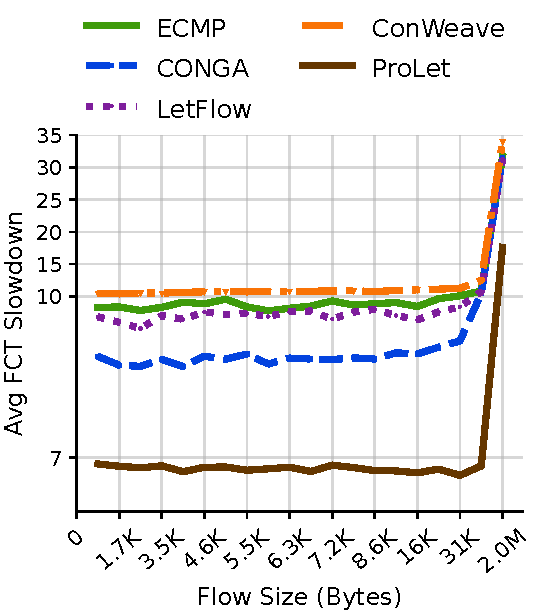
\includegraphics[width=0.46\columnwidth]{AVG_32_ALI.pdf}}
    \hfill
    \subfloat[\textbf{P99 FCT.}\label{fig:fct_fat_tree_p99}]{
        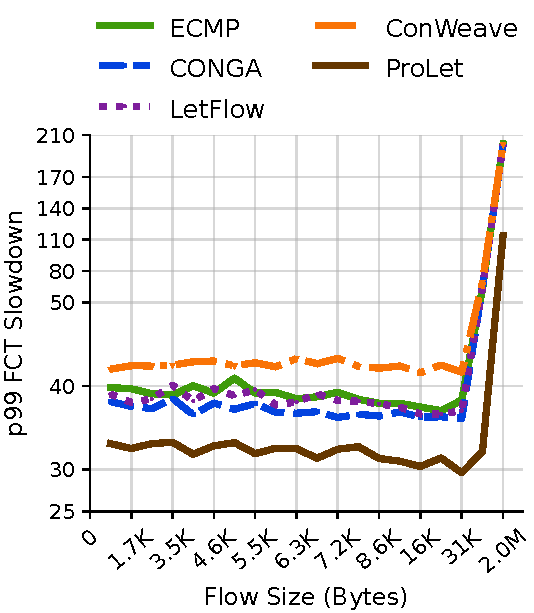
\includegraphics[width=0.46\columnwidth]{P99_32_ALI.pdf}}
    \caption{Historical reference: average and tail FCT slowdowns from the earlier prototype for AliStorage on Fat-Tree-32 (80\% load, all-to-all). These curves do not evaluate the revised exploration-first design.}
    \label{fig:FCT_large_top}
\end{figure}

\subsection{Workload Generation} 
To demonstrate the generalization of DuoGran, we evaluate DuoGran in workloads with different flow size distribution and traffic pattern. The existing workloads are divided into two application scenarios.

\noindent
\textbf{Cloud storage:} We use Meta Haddoop and AliStorage as representative cloud storage workloads. To generate the workload, we reuse the workload generation module in HPCC \cite{HPCC} and ConWeave \cite{Conweave}. This module employs an all-to-all traffic pattern with hosts selected uniformly at random. Flow arrivals follow a Poisson distribution with inter-arrival times following the exponential distribution. With an average network load of 80\%, each host generates traffic at 40\% of its uplink bandwidth to accommodate the $2{:}1$ oversubscription ratio.

\noindent
\textbf{Distributed model training:} We construct a model-driven training workload using AICB's \texttt{LLaMA\_7B} benchmark preset and SimCCL. The 128 hosts, each equipped with one GPU, are organized into eight model replicas, each occupying the 16 hosts connected to the same leaf. Each model is partitioned into four pipeline stages, with four-way tensor parallelism (TP) within each stage. A data parallelism (DP) group connects the corresponding hosts across all eight replicas, yielding 16 DP groups. This placement keeps frequent TP collectives and PP activation/gradient transfers within a leaf, while restricting inter-leaf training traffic to DP synchronization.

AICB generates the model operations and pipeline schedule from the model, batch, and parallelism configuration. SimCCL expands collective communications such as Ring Allreduce into point-to-point flows with dependencies. Our converter maps communication endpoints to physical hosts and constructs a directed acyclic graph (DAG) containing \texttt{compute}, \texttt{send}, and synchronization events. The DAG edges encode execution dependencies. The \texttt{send} nodes indicate communication events with the specified source, destination, and payload size. We estimate the duration of \texttt{compute} nodes using ASTRA-sim's Roofline model with A100 parameters. 

During NS-3 replay. Computing completion and acknowledgment of an entire flow release dependent events, and an event becomes ready when all its predecessors have completed. \texttt{Compute} events are executed through a per-host FIFO with one active compute event per GPU. \texttt{Send} events are submitted to the existing RDMA stack, which multiplexes packets from concurrent flows.

\subsection{Earlier Results and Evaluation Needs}
\label{sec:result}
\noindent
\textbf{Reduction in PFC pause frames:} Since RDMA relies on PFC to ensure losslessness, the frequency of pause frames serves as a direct indicator of network-wide congestion \cite{PFC_inidcator}. Table~\ref{Table:stats} compares the total PFC pause frame count in a 128-host Spine-Leaf topology in millions. These historical baseline measurements do not quantify the revised policy's effect.
\begin{table}[t]
\centering
\setlength{\tabcolsep}{3pt}
\caption{Historical reference: flowlet packet-count statistic (>100 packets) and PFC pause frames from the earlier prototype under AliStorage on Spine-Leaf-128.}
\begin{tabular}{lcc}
\hline
\textbf{Scheme}   & \textbf{Avg. Packet Count}  & \textbf{PFC Frames (M)}\\
\hline
ECMP~\cite{ECMP}            & \textemdash   & 12.7 \\
CONGA~\cite{Conga}      & 638           & 9.8\\   
LetFlow~\cite{Letflow}  & 612           & 12.9\\
ConWeave~\cite{Conweave}          & \textemdash   & 0.8 \\
\hline
\end{tabular}
\label{Table:stats}
\end{table}



\noindent
\textbf{Reduction in average and tail FCT slowdown:} The earlier prototype reported reductions in average and P99 FCT slowdown of up to 69\% and 79\%, respectively, in Fig.~\ref{fig:FCT_large_top}. Its analysis considered the following limitations of the baselines.
\begin{enumerate*}[label=(\roman*)]
    \item \textbf{Static-timeout schemes:} A fixed timeout may miss usable gaps even when the workload contains sufficiently large inter-packet gaps; the relevant comparison is between each gap and the applicable rerouting threshold.
    \item \textbf{Subflow-based schemes:} While ConWeave's subflow-based rerouting is effective in a 128-host Spine-Leaf topology, it is sensitive to network scale. In a 32-host topology with fewer equal-cost paths, mice flows suffer from persistent hash collisions, and rerouting them prolongs their FCT.
\end{enumerate*}







\subsection{Effect of Protected Subflow Rerouting}
\label{sec:subflow_fct_ablation}

We compare timeout-only DuoGran against DuoGran with the protected subflow branch in Sec.~\ref{sec:selective_handoff} enabled. Both configurations use the same 52,469-flow Hadoop trace, seed 1, and 4,096-byte packet payload on the 128-host, 100-Gbps Spine--Leaf topology with 2:1 oversubscription and 80\% network offered load. Flows arrive over 10~ms, and the statistics include all completed flows, including the drain period. Both configurations retain the same initial exploration, probe-timeout and ECN congestion detection, and fastest-available-path selection. If the ordinary timeout check fails, the enabled branch permits an early reroute when the current path is invalid, the arrival gap exceeds $2~\mu\mathrm{s}$, and a faster available candidate passes the predicted-improvement check, using destination-ToR buffering during the handoff.

\begin{figure}[t]
    \centering
    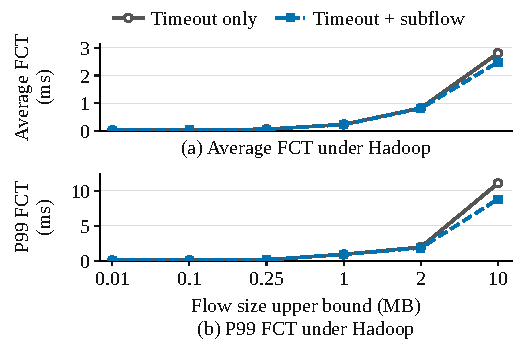
\includegraphics[width=\columnwidth]{figures/duogran_timeout_subflow_fct.pdf}
    \caption{Average and P99 FCT with and without protected subflow rerouting under Hadoop. Flow-size ticks denote bin upper bounds; 1 MB equals $10^6$ bytes.}
    \label{fig:subflow_fct_ablation}
\end{figure}

Figure~\ref{fig:subflow_fct_ablation} shows that the gains are concentrated in large flows. For the 800 flows in the 2--10-MB bin, protected subflow rerouting reduces average FCT from 2.804 to 2.481~ms (11.50\%) and P99 FCT from 11.093 to 8.830~ms (20.40\%). Across all flows, average and P99 FCT decrease by 6.18\% and 5.40\%, respectively. The benefit is not uniform: for flows up to 10~KB, average and P99 FCT increase by 2.36\% and 1.78\%; for 10--100-KB flows, they increase by 3.94\% and 1.87\%. This single-seed comparison supports using protected subflow rerouting to improve large-flow completion times, with a modest small-flow penalty in this workload.

\begin{figure}[t]
    \centering
    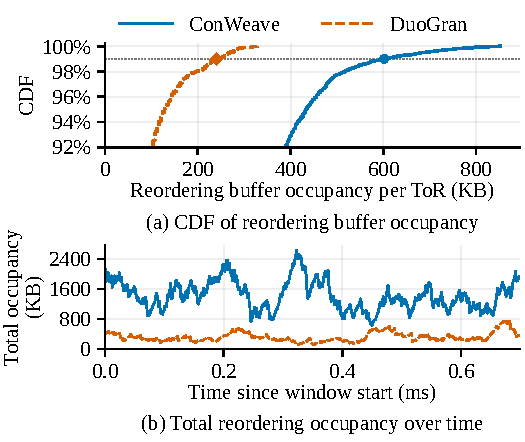
\includegraphics[width=0.85\columnwidth]{figures/dst_reordering_buffer_cdf.pdf}
    \caption{Destination-ToR reordering-buffer occupancy in the 4.0--4.7-ms window of the 5-ms workload: (a) per-ToR CDF, including zero samples, with the 92--100\% range shown and P99 marked; (b) simultaneous total across eight ToRs, with time relative to the window start. One KB equals 1,000 bytes.}
    \label{fig:dst_buffer_occupancy}
\end{figure}

\subsection{ConWeave Reordering Observations}
\label{sec:conweave_reordering}



\begin{table}[!b]
    \centering
    \caption{Network-wide ConWeave reordering counts over the complete run (20-ms traffic generation; 20.8-ms observation).}
    \label{tab:conweave_reordering_observation}
    \footnotesize
    \renewcommand{\arraystretch}{1.15}
    \begin{tabularx}{\columnwidth}{@{}Xr@{}}
        \toprule
        \textbf{Metric} & \textbf{ConWeave} \\
        \midrule
        Total reordering episodes & 36,480 \\
        Timeout-based releases & 18 \\
        Out-of-order packets detected at RNIC (arrival count) & 1,063 \\
        \bottomrule
    \end{tabularx}
    \par\smallskip
    \begin{minipage}{\columnwidth}
    \footnotesize TAIL-based releases: 36,462; unreleased episodes at end: 0. Counts cover the full input logs, including the drain period. The out-of-order count includes arrivals with a sequence number greater than the RNIC's next expected sequence number; repeated arrivals can be counted more than once.
    \end{minipage}
\end{table}

Table~\ref{tab:conweave_reordering_observation} separates reordering episodes, timeout-based releases, and out-of-order arrivals at the receiver RNIC. Of 36,480 episodes, 36,462 end through TAIL-based release and 18 through timeout-based release; the receiver RNIC detects 1,063 out-of-order arrivals. Residual reordering occurs in this run, but the aggregate counts do not establish that timeout-based release caused these out-of-order arrivals. These counts describe reordering behavior; they do not measure destination-buffer occupancy or packet waiting time.



\subsection{Destination-ToR Reordering-Buffer Occupancy}
\label{sec:dst_buffer_occupancy}

We compare ConWeave~\cite{Conweave} and DuoGran using the same 78,171-flow AliStorage trace and random seed on the 128-host Spine--Leaf topology. Flows arrive over 5~ms with a 4,096-byte payload. We sample all eight ToRs at $1~\mu\mathrm{s}$ intervals over $[4.0,4.7)$~ms after traffic starts, yielding 5,600 samples, including zero occupancy. The CDF shows per-ToR occupancy, while the time series shows the aggregate across all eight ToRs. Occupancy includes buffered packet headers but excludes per-connection metadata.

Figure~\ref{fig:dst_buffer_occupancy}(a) shows lower per-ToR reordering-buffer occupancy for DuoGran in this run. Its P99 occupancy is 240.35~KB, compared with 601.77~KB for ConWeave, a reduction of approximately 60.1\%. Mean per-ToR occupancy is 40.19~KB versus 178.85~KB, a reduction of 77.5\%. The maximum sampled per-ToR occupancy is 327.38~KB versus 851.55~KB. These are maxima over sampled states, not exact event-level peaks or simultaneous network-wide totals. Figure~\ref{fig:dst_buffer_occupancy}(b) complements the CDF by showing the temporal variation in aggregate occupancy across all eight ToRs during the same window.

\noindent\textbf{Why occupancy can be lower:} DuoGran selectively uses destination buffering rather than initiating a protected handoff on every path change. Outside an active protected handoff, traffic that can use the ordinary delay-aware timeout rule does not start a new destination reordering session. In particular, a flow whose current path remains available cannot initiate the early-rerouting branch. This preserves the natural-gap-based mechanism for paths not marked congested and limits the traffic that requires explicit buffering. Ordinary timeout reroutes occurring during an already active handoff remain protected until that handoff completes.

For a current path marked invalid, DuoGran first tries the ordinary timeout rule. Only if that rule rejects the switch does it consider early rerouting, and then only when the existing same-flow arrival gap exceeds $2~\mu\mathrm{s}$ and a faster available candidate passes the predicted-improvement check. Thus, even congestion-driven early rerouting waits for a natural gap instead of switching immediately on every congestion indication. The gap gives previously transmitted packets a head start, while the gap and benefit checks restrict the number of handoffs that can create new buffering demand. New-path packets that arrive before the corresponding old-path END marker are held at the destination ToR and released once the required boundaries have completed.

These mechanisms are consistent with the lower occupancy observed here, but this experiment does not isolate their individual contributions. In particular, END is injected at the time of rerouting and still traverses the old path; an existing arrival gap does not guarantee a shorter wait for END. The observation window excludes the post-generation drain, but it covers only one interval and one random seed. Longer runs, additional observation windows, multiple seeds, and ablations of the early-rerouting gap threshold are needed to establish how much of the reduction comes from selective buffering versus reuse of natural gaps.

\noindent
\textbf{Required revised evaluation:} Repeat average and P99 FCT, PFC, and packet-reordering measurements with the current implementation and matched traffic seeds and payload settings. Compare rerouting enabled and disabled while keeping initial exploration identical. Report accepted path changes and the distributions of packet gaps, computed timeouts, predicted improvements, and OWL sample ages. These distinguish identifying a sufficiently large gap from actually admitting a beneficial path change. Sparse new-flow arrivals, delayed feedback, and rapid OWL changes should be examined because the current policy cannot guarantee fresh measurements on unused paths or bound unobserved queue changes.

\begin{figure*}[!t]
    \centering
    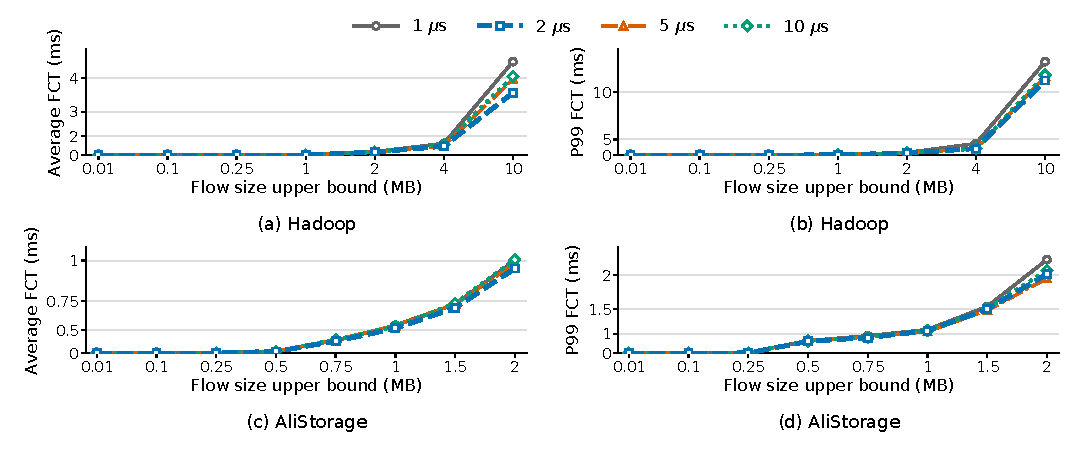
\includegraphics[width=\textwidth]{figures/duogran_gap_sensitivity.pdf}
    \caption{Sensitivity to the early-rerouting gap threshold: average and P99 FCT under Hadoop (a, b) and AliStorage (c, d). Legend values are gap thresholds. Flow-size ticks indicate workload-specific bin upper bounds; 1 MB equals $10^6$ bytes. The vertical axes use a quadratic scale (position proportional to FCT$^2$), while tick labels show actual FCT in milliseconds.}
    \label{fig:gap_sensitivity}
\end{figure*}

\subsection{Sensitivity to the Early-Rerouting Gap Threshold}
\label{sec:gap_sensitivity}

We vary the arrival-gap threshold for protected early rerouting over 1, 2, 5, and 10~$\mu$s, keeping the ordinary path-pair timeout rule, probe-timeout and ECN congestion detection, and fastest-available-path selection unchanged. The experiments use the 128-host, 100-Gbps Spine--Leaf topology with 2:1 oversubscription, 80\% network offered load, and a 4,096-byte packet payload. Each workload uses the same input trace across all four configurations: 52,469 Hadoop flows or 156,777 AliStorage flows, generated over 10~ms with seed~1. Statistics include all completed flows and the drain period. Within each workload, all configurations use identical size bins and flow cohorts; each bin's P99 is computed directly from its individual flow FCTs.

Figure~\ref{fig:gap_sensitivity} shows that the effect depends on flow size and workload. For Hadoop flows of 4--10~MB, the 1-$\mu$s configuration has an average FCT of 4.408~ms, compared with 3.604~ms at 2~$\mu$s, a 22.3\% increase. For the 2--4-MB bin, its P99 rises from 3.266 to 4.300~ms (31.7\%). AliStorage exhibits smaller differences and a different ranking in some bins: for 1.5--2-MB flows, the 5-$\mu$s configuration has a P99 of 1.957~ms, versus 2.012~ms at 2~$\mu$s. Across all flows, 2~$\mu$s gives the lowest absolute average and P99 FCT among the four tested settings for both workloads, but it does not minimize every per-size metric. These single-seed results support retaining 2~$\mu$s as the default in this configuration; they do not establish a universal optimum. The last two Hadoop bins contain 402 and 398 flows, respectively, so their P99 estimates depend on only a few extreme samples.

% Start the conclusion below the final evaluation figure on the next column/page.
\newpage
\section{Conclusion and Future Work}
DuoGran combines exploration-first path assignment with uniform, delay-change-aware flowlet rerouting in lossless RDMA networks. New flow entries first explore eligible paths; existing flows consider only the lowest-OWL available path and switch when predicted improvement and packet-gap conditions both hold. All flows share per-path feedback without a host classifier, a fixed flow-size threshold, or class-dependent routing. A per-destination summary tree supports path selection without storing a timeout per flow. Future work includes evaluating the revised policy, quantifying its reordering behavior under stale feedback, and validating a hardware implementation.


% IEEE journal bibliography style
\bibliographystyle{IEEEtran}

\bibliography{reference}

\end{document}
